are also illustrated in figure \ref{brillouin_zone_001},  are:
\begin{wrapfigure}{r}{0.3\linewidth}
	\centering
	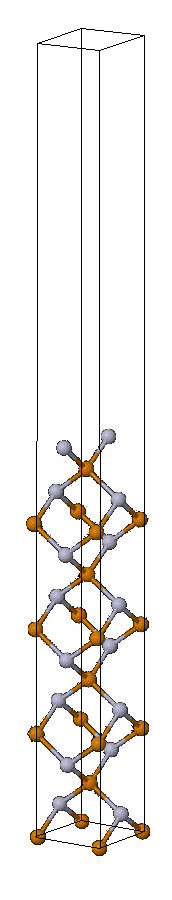
\includegraphics[width=0.6\linewidth]{hgte_16layer_supercell.jpg}
				\caption{Supercell with 16 layers and additional space at the top, representing the vacuum. (like in \cite{Graz}) } \label{16layer_supercell}
\end{wrapfigure} 

\blindtext
%\begin{description}
%	\item[bla] \blindtext
%	\item[bla] \blindtext
%	\item[bla] \blindtext
%	\item[bla] \blindtext
%	\item[bla] \blindtext
%	\item[bla] \blindtext
%	\item[bla] \blindtext	
%\end{description}
\paragraph{bla}\blindtext\paragraph{bla}\blindtext\paragraph{bla}\blindtext\blindtext




%\blindtext\blindtext\blindtext\blindtext\blindtext
%%% Local Variables:
%%% mode: latex
%%% TeX-master: "main_BA2.0"
%%% End: